%
% Acta Acustica united with Acustica -- Instructions for Authors, 2017-03-01
%
\documentclass[twocolumn]{article}

%%%%%%%%%%%%%%%%%%%%%%%%%%%%%%%%%%%%%%%%%%%%%%%
%% Comment / uncomment for one or two column(s) fomat
%\documentclass{article}

\usepackage[modulo,switch]{lineno}
\modulolinenumbers[1]
%%%%%%%%%%%%%%%%%%%%%%%%%%%%%%%%%%%%%%%%%%%%%%%
%% Comment / uncomment for showing line numbers

\usepackage[utf8]{inputenc}
\usepackage{amsmath}
\usepackage{amssymb}
\usepackage{graphicx}
\usepackage{float}
\usepackage{setspace}
\usepackage{enumitem}
\usepackage{titlesec}
\usepackage{lipsum}% just to generate text for the example
\usepackage{nameref}
\usepackage{listings}
\usepackage{xcolor}
\usepackage{caption}
\usepackage{subcaption}
\lstset { 
	language=C++,
	backgroundcolor=\color{black!5}, % set backgroundcolor
	basicstyle=\footnotesize,% basic font setting
}
%put code snippet
\usepackage{color}
\usepackage{listings}
\definecolor{codegreen}{rgb}{0,0.6,0}
\definecolor{codegray}{rgb}{0.5,0.5,0.5}
\definecolor{codepurple}{rgb}{0.58,0,0.82}
\definecolor{backcolour}{rgb}{0.95,0.95,0.92}

\titlespacing*{\section}
{0pt}{5pt}{5pt}
\titlespacing*{\subsection}
{0pt}{5pt}{5pt}

\makeatletter\@ifundefined{date}{}{\date{}}
\makeatother
\setstretch{1}
\setlist[itemize]{noitemsep}

\paperheight297mm \paperwidth210mm
\textwidth177mm  \textheight290mm  \oddsidemargin 8mm
\evensidemargin\oddsidemargin \hoffset-20mm \voffset-40mm
\topmargin0pt \headheight8mm \headsep2mm \topskip0mm
\footskip7.5mm \columnsep8mm \arraycolsep2pt \parindent5pt
\renewcommand{\abstractname}{Abstract} 

\begin{document}
	
	\title{Final Project: Syrup Dispenser}
	
	\author{Franziska Rothen - franziska.rothen@students.unibe.ch - \today}
	
	\maketitle\thispagestyle{empty}
	
	\section*{Abstract}
	For the final project in the course programming of microcontrollers the goal was to implement a syrup dispenser in collaboration with another student. The following functionalities on my side were foreseen: Navigation through the LCD menu via joystick, detection of the size of the glass with a weighing scale (choice between a small and big glass), choice of syrup percentage via potentiometer, communication with the second microcontroller; giving orders to open and close valves as well as moving the glass to three predefined positions. 
	
	\section{Materials and Methods}
	For the following sections, only the subpart of the project concerning my work is addressed.
	
	The code was implemented on a Nucleo-F446RE (using the software STM32CubeIDE 1.7.0$^1$) with the addition of the MBED-016 multi-purpose PCB. This board contains the LCD and joystick for the menu navigation and the potentiometer to choose the percentage. Further, the Saleae logic analyzer was used to analyze some signals for debugging purposes. Lastly, the HX711 24-Bit Analog-to-Digital Converter$^2$ with a load cell of 1kg was used as a weighing scale.	
	
	\subsection{Configurations}
	On the STM32CubeIDE the following configuration was implemented:
	
	Pin PA0 (the potentiometer) was set up as ADC in scan conversion mode and with a resolution of 12 bits.
	
	PA9/PA10 and PA2/PA3 served as USART to communicate with the second microcontroller involved in this project and for debugging purposes respectively. 
	
	For the LCD, SPI communication with the following pins were used: PA5 for the clock signal (SCK), PA6 as reset pin, PA7 for master out, slave in (MOSI), PA8 for the register select (A0=0: Instruction, A0=1: Data) and finally PB6 for the chip select signal (CS\_N). The SPI is configured as Half-Duplex Master.
		
	Next, the joystick was implemented as GPIO\_EXTI on pin PB5. 
	
	Finally, the HX711 data and clock lines were set to pins PB8 and PB9 as GPIO input and output respectively.
.
	The internal timer TIM1 was activated with the following settings:\newline
	$Prescaler = 15'999$; $Period = 49$ \newline
	Which results in an update (reset) event at a rate of 20Hz, according to equation 1:
	\begin{equation}
	UpdateEvent = \frac{Timer_{Clock}}{(Prescaler+1)(Period+1)}
	\end{equation}

	 
	\subsection{Implementation}
	In general, both a header and source file were created containing functions for each component individually. 
	\subsubsection{Setup}
	After the initialization of all the peripherals, the scale is set up with an initialization function. The LCD is initialized as well and displays a welcome message. All the files and code for the interaction with the LCD was provided by Prof. Dr. Patrick Arnold.
	
	Additionally, a command is transmitted to the second microcontroller to make it home the stepper motor. Refer to chapter \ref{sec:comm} \nameref{sec:comm} for more information on the communication between the two microcontrollers.
	
	For the setup of the weighing scale, refer to chapter \ref{sec:weigh} \nameref{sec:weigh}.
	
	\subsubsection{Menu} \label{sec:menu}
	The functionality of the menu is implemented in the while loop. The variable called $step$ keeps track of the progress in the menu. The increment happens with an external interrupt of the corresponding GPIO (joystick). To handle bouncing, a timer (TIM1) is started when the button is pressed. Only after the elapse of the timer period the button is checked. If the pin is reset, only then will the $step$ variable be incremented by 1.
	
	These are the steps in the menu with their intended functionality:
	
	\begin{enumerate}
		\item Display of the first prompt on the LCD: The user is asked to press the joystick to continue in the menu.
		\item Display of the second message: The user is asked to place a glass on the scale.
		\item With the function $getWeight()$, the current weight on the scale is measured and displayed on the LCD.
		\item The weight is compared to a predefined value to distinguish and state the size of the glass chosen.
		\item In this step, the potentiometer is initialized. Its range of values is divided into 20 equal parts which represent a syrup percentage of $5\%$ up to $20\%$. The current value is displayed on the LCD.
		\item The potentiometer is de-initialized since it is no longer needed. The final choice of syrup percentage is displayed.
		\item Now, a command is sent to the other microcontroller to move the glass to the next position, where the syrup is dispensed in the glass. Consequently, the syrup-valve is opened. The variable $step$ is increased by 1 to immediately move on to the next step.
		\item While the glass is filled with syrup, the weight on the scale is acquired and the message "Filling..." is displayed on the LCD. As soon as the weight exceeds the $volume*percentage$ (where the volume is the weight of the small or big glass respectively if it was filled completely with syrup), the flag $isFull$ is set to a logic high. 
		As soon as $isFull$ is high, the following commands are send to the second microcontroller: 
				
		\newpage
		\vspace*{40px}
		
		\begin{enumerate}
			\item Close the syrup-valve
			\item Move the glass to the next position
			\item Open the water-valve
		\end{enumerate}
		$Step$ is incremented by 1 and $isFull$ is reset.
		\item The same procedure is repeated for the filling of water. Rather than comparing the weight to a percentage of the full glass, the $isFull$ flag is set to a logic high when the weight exceeds the volume of the glass completely filled with water. As soon as the water has reached the desired level meaning $isFull$ is true, the following actions are commanded to the other microcontroller:
		\begin{enumerate}
			\item Close the water-valve
			\item Move the glass to the starting position
		\end{enumerate}
		$Step$ is incremented once again by 1.
		\item "Cheers!" is displayed on the LCD.

	\end{enumerate} 
	
	\subsubsection{Weighing Scale} \label{sec:weigh}
	For the HX711, already existing open source functions were used$^3$. The HX711 header and source files were imported into the project folder. The ADC itself is set up as seen in figure \ref{fig1}. The power supply and ground are connected to the +5V and the ground pins, the PD\_SCK and DOUT to pins PB8 and PB9 on the Nucleo board respectively. 
	
	\begin{figure}[H]
		\centering
		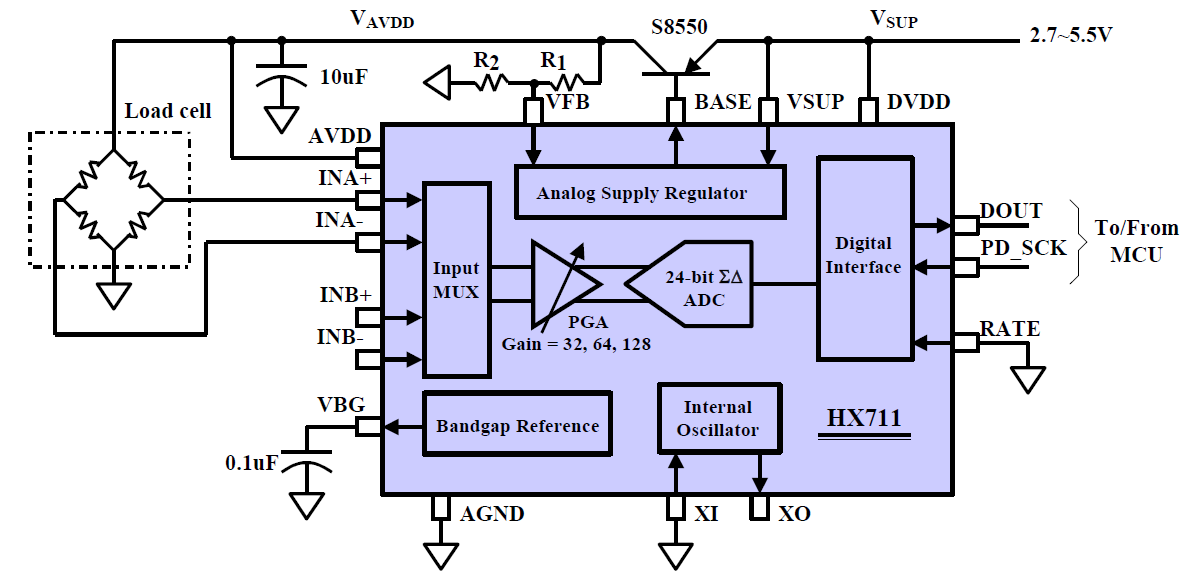
\includegraphics[width=85mm]{hx711.PNG}
		\caption{Typical weigh scale application block diagram of the HX711}
		\label{fig1}
	\end{figure}

	The acquisition of the data works solely through the data and clock pins. 
	The data channel works as follows: As soon as it is ready to transmit data it will switch from a logical high to low. Once ready it can take up to 27 clock impulses for each of which it returns a bit-value. This way, the output adds up to a value representing the weight on the scale (see figure \ref{fig2}).

	\begin{figure}[H]
	\centering
	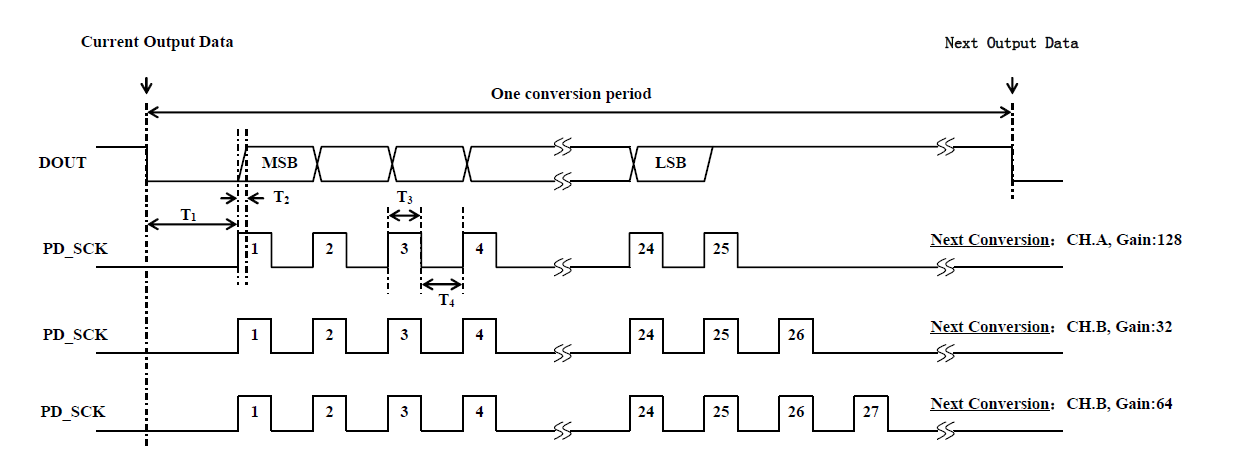
\includegraphics[width=85mm]{hx712.PNG}
	\caption{Data output, input and gain selection timing and control}
	\label{fig2}
	\end{figure}

	\newpage
	\vspace*{40px}	
	
	By generating 25 input pulses on the clock, the gain is set to 128. 
	The scale was initially calibrated by measuring the value of an empty scale and then after placing 1kg on it. The return value of the function
	\begin{lstlisting}[language=C++]
 hx711_weight(hx711_t *hx711, uint16_t sample)
	\end{lstlisting} is then adjusted to give the correct result by first subtracting the offset for 0g and then scaling the value at 1kg to correspond to 1000g. In addition, the values are averaged over 10 samples in this function to get a more steady result.
	
	\subsubsection{Communication}  \label{sec:comm}
	
	The communication between the two microcontrollers is done using USART as stated before. The following characters are used for the different commands: \newline\newline
	\begin{tabular}{|c|c|}
		\hline
		Message & Function \\ 
		\hline\hline 
		l &  Homing the motor\\ 
		\hline 
		b & Move the glass to the next position\\ 
		\hline 
		t&  Open the syrup-valve\\ 
		\hline 
		z&  Close the syrup-valve\\ 
		\hline 
		g& Open the water-valve \\ 
		\hline 
		h& Close the water-valve \\ 
	\hline 
		m& Move the glass to starting position \\ 
	\hline 
	\end{tabular} 
	
	\vspace*{5px}	
	
	
	\section{Results}
	The menu on the LCD works as planned and shows the correct weights and syrup percentages. The percentage of the syrup can be selected ranging from 5\% to 25\% as seen in figure \ref{fig5}:
	
	\begin{figure}[H]
		\centering
		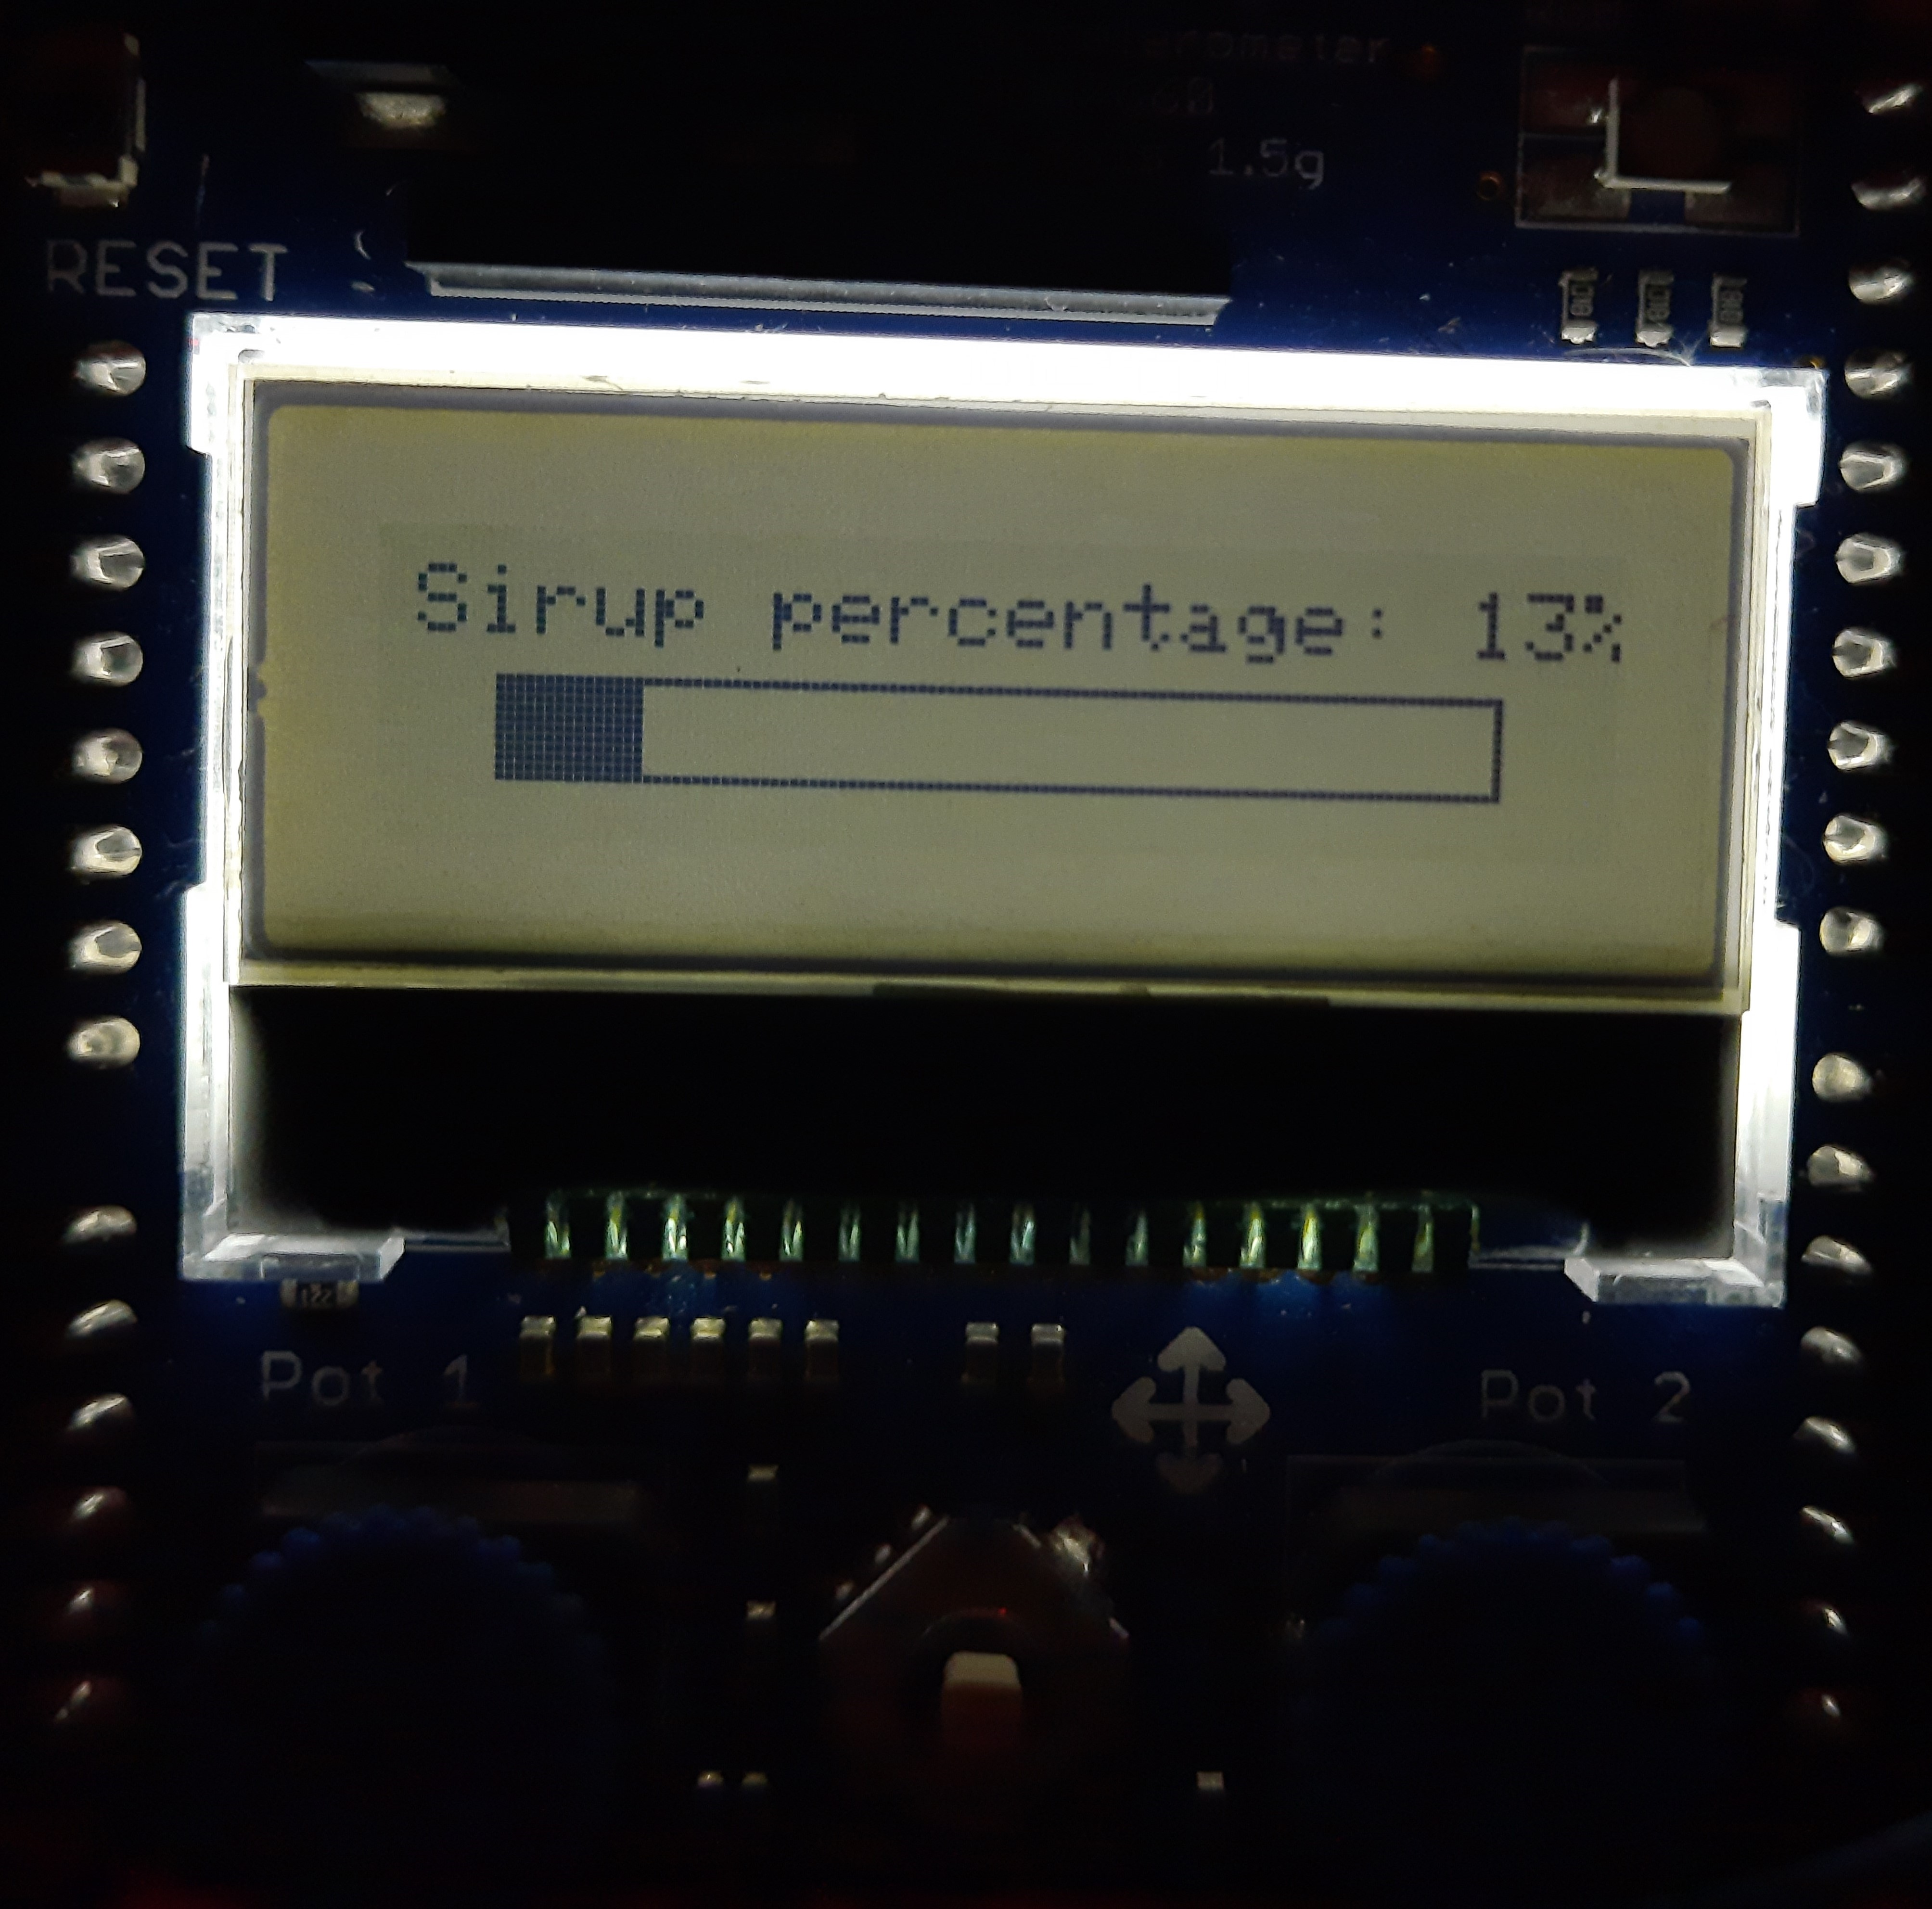
\includegraphics[width=75mm]{lcd.jpg}
		\caption{Picture of the LCD while selecting the percentage of the syrup.}
		\label{fig5}
	\end{figure}
	
	\newpage
	\vspace*{40px}
	
	For my initial approach, problems occurred with bouncing of the joystick when navigating in the menu:
	
	\begin{figure}[H]
		\centering
		\begin{subfigure}[b]{\columnwidth}
			\centering
			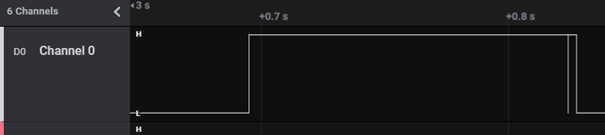
\includegraphics[width=\columnwidth]{debounce1.PNG}
			\caption{}
			\label{subfig3.1}
		\end{subfigure}
		 
		\begin{subfigure}[b]{\columnwidth}
			\centering
			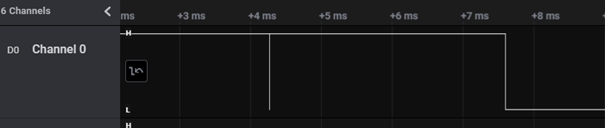
\includegraphics[width=\columnwidth]{debounce2.PNG}
			\caption{}
			\label{subfig3.2}
		\end{subfigure}
		\caption{Measurements taken from the output signal of the joystick button. (a) Output signal captured for one push and release of the joystick. (b) Zoom on the bouncing of the signal.}
		\label{fig3}
	\end{figure}

	A signal artifact appears that lasts less than 4ms. It causes the detection of two rising edges instead of just the one. Solution to this problem is de-bouncing and is described in chapter \ref{sec:menu}. The result is a clean signal resulting in only one rising edge when the joystick is pressed.
	\newline
	
	As for the timer signal, the following data and clock signal was measured:
	
	\begin{figure}[H]
	\centering
		\begin{subfigure}[b]{\columnwidth}
			\centering
			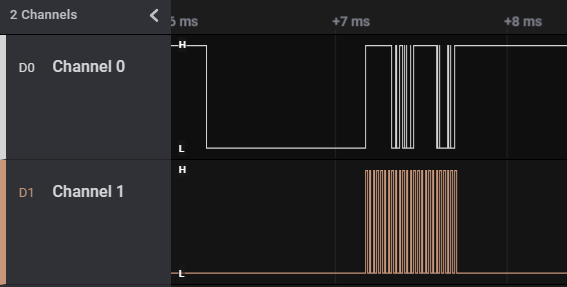
\includegraphics[width=\columnwidth]{scale1.PNG}
			\caption{}
			\label{subfig4.1}
		\end{subfigure}
		
		\begin{subfigure}[b]{\columnwidth}
			\centering
			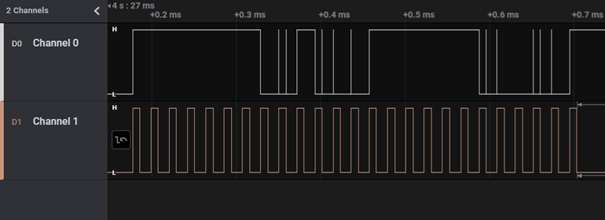
\includegraphics[width=\columnwidth]{scale2.PNG}
			\caption{}
			\label{subfig4.2}
		\end{subfigure}
		\caption{The data (Channel 0) and clock signal (Channel 1) are measured on the respective pins for one measurement of the weighing scale. (a) Overview of one signal measurement. (b) Zoom on the clock input pulses and the corresponding output data.}
		\label{fig4}
	\end{figure}
	
	One millisecond after the data signal (Channel 0) switches to low and is therefore ready, the clock signal transmits 25 impulses (Channel 1). The bits captured in this manner represent the weight on the scale. 
	
	\newpage
	\vspace*{40px}
	
	\section{Discussion}
	All intended functions were implemented successfully. Nonetheless, there are a few things that could be improved on continuation of this project:
	
	\begin{enumerate}
		\item Menu navigation: As of now it is only possible to move forward in the menu. What could be a nice addition is to be able to step back to change the percentage for example or check some information displayed in an earlier stage of the menu. The implementation should be fairly easy since the same principle applies as for moving forward: on the signal of a pushed button, the variable $step$ as seen in chapter \ref{sec:menu} will be decremented rather than incremented.
		
		\item An approximation that is made in the calculations is that syrup and water possess the same density. In a real application, this should be changed since the density of syrup can be much higher than water, making the disposed amount faulty. For the syrup disposal this change could easily be made by just adjusting the total weight of the glass when filled with syrup completely. The filling of the water is currently done by just checking the weight of the glass completely filled with water. So if the density of syrup differs from that of water, the total weight would vary depending on the percentage chosen. This would have to be included in the calculation and the weight would have to be adjusted accordingly.
	\end{enumerate} 

	
	\section*{References}
	[1] STM32 Nucleo-64 boards (MB1136), https://www.st.com, 2017 \newline 
	[2] Datasheet: HX711 - 24-Bit Analog-to-Digital Converter (ADC) for Weigh Scales
	\newline
	[3] https://github.com/nimaltd/HX711
\end{document}